\cotefile{35}
\scanpage{2}
\noindent\hfill\margin{\handwritten{\unsure{zurück} \unsure{an|au} G.}}\par

\noindent SGA 7\qquad Groupe de Monodromie en Géométrie Algébrique

\reversemarginpar
\noindent\margin{\handwritten{\unsure{Gr|Gro}}}I\quad G\deleted{\unsure{ad|ed}}énéralités sur le g\deleted{\unsure{o}}roupe de monodromie locale. Le théorème de monodromie par voie arithmétique.

\noindent\margin{\handwritten{Gr}}II\quad Cas d'action\deleted{s} résoluble\deleted{s} d'ungroupe fondamental (variante du \deleted{groupe} théorème de monodromie).

\noindent\margin{\handwritten{Gr}}III\quad Le théorème de monodromie par voie géométrique.\normalmarginpar
\margin{\handwritten{\figure{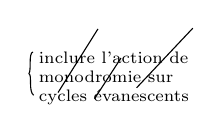
\begin{tikzpicture}[x=1cm,y=1cm,scale=.86,transform shape]
\node[anchor=north west,align=left,inner sep=0pt,font=\scriptsize] at (.14,.06)
{\deleted{\unsure{inclure} l'action \unsure{de}}\\
 \deleted{\unsure{monodromie} sur}\\
 \deleted{\unsure{cycles} évanescents}};
\draw (.06,.05) .. controls (-.01,.03) and (.04,-.22) .. (0,-.27)
 .. controls (.05,-.29) and (-.01,-.53) .. (.07,-.59);
\draw (.43,-.55)--(1.02,.39) (.97,-.64)--(1.36,-.04) (1.59,-.48)--(2.42,.40);
\end{tikzpicture}}}}

\reversemarginpar
\noindent\margin{\handwritten{Gr}}IV\quad Propriétés générales des groupes de cycles évanescents. Cas des points singul\deleted{\unsure{ei|ee}}iers isolés de la fibre spéciale.

% slanted
\noindent\margin{\handwritten{Gr\par
\figure{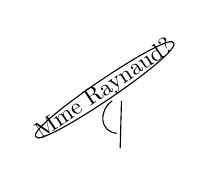
\begin{tikzpicture}[scale=.84,transform shape]
\begin{scope}[rotate=34,transform shape]
\node[inner sep=1.1pt] (q) {Mme Raynaud?};
\draw (q.west) .. controls (q.north west) and ([xshift=3pt]q.north east) .. (q.east)
 .. controls (q.south east) and ([xshift=-3pt]q.south west) .. (q.west);
\end{scope}
\draw (q.south) .. controls +(-.21,-.15) and +(-.26,.02) .. ++(.07,-.49);
\draw ([xshift=4pt]q.south) -- ++(-.02,-.72);
\end{tikzpicture}}}}V\quad Groupe de monodromie opérant sur le groupe fondamental: théorèmes d'action modérée et d'action essentiellement modérée.

\noindent\margin{\handwritten{Mme Raynaud\par\deleted{Mme Raynaud}}}\deleted{VI}\handwritten{\inserted{App.}}\quad Application: présentation finie des groupes fondamentaux géométrique\unsure{s}

\noindent\margin{\handwritten{\uline{\unsure{Rim}}}}\handwritten{\inserted{$\underline{\overline{\mathrm{VI}}}$\quad \unsure{Modules} formels (\unsure{ist} bei Deligne)}}

\noindent\margin{\handwritten{Gr}}VII\quad Biextensions de faisceaux de groupes.

\noindent\margin{\handwritten{Gr}}\handwritten{\inserted{$\underline{\overline{\mathrm{VIII}}}$\quad Extensions et \unsure{biextensions} de \unsure{schémas} \unsure{en groupes} \unsure{par} $\unsure{G_m|\mathbb{G}_m}$}}

% The outlined typescript above this line has a downward point between the two words.
\noindent\margin{\handwritten{Gr}}\deleted{\unsure{VIII}}\handwritten{$\underline{\overline{\mathrm{IX}}}$}\quad Application\handwritten{s} au modèle de Néron: \deleted{le} théorème \inserted{d'orthogonalité, théorème} de réduction semi-stable.\handwritten{\tikz[baseline]{\draw[line cap=round] (.01,.045)--(.045,.020) (.11,.035)--(.155,.025) (.23,.059)--(.28,.046);}}

\noindent\margin{\handwritten{\deleted{Deligne}}}
\figure{\resizebox{\linewidth}{!}{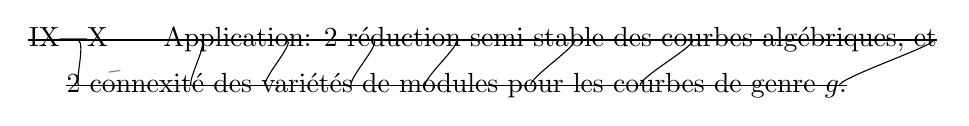
\begin{tikzpicture}
\node[anchor=west,inner sep=0pt] (a) at (0,0) {\deleted{\unsure{IX|X}}\qquad \deleted{Application: {\deleted{\illegible{2}}} réduction semi-stable des courbes algébriques, {\deleted{\unsure{et}}}}};
\node[anchor=west,inner sep=0pt] (b) at (.48,-.58) {\deleted{{\deleted{\illegible{2}}} \tikz[overlay]{\draw[gray] (.24,.26)--(.39,.28);}connexité des variétés de modules pour les courbes de genre $g$.}};
\draw (a.west) -- (a.east);
\draw (b.west) -- (b.east);
\foreach \p/\q in {.055/.016,.19/.16,.285/.255,.38/.365,.47/.46,.60/.595,.73/.735,.995/.99}
{\path (a.west) -- (a.east) coordinate[pos=\p] (t);
 \path (b.west) -- (b.east) coordinate[pos=\q] (u);
 \draw (t) .. controls +(0.09,-.05) and +(-.04,.09) .. (u);}
\end{tikzpicture}}}

% archive sheet number: 1
